\section{Grad-Shafranov Equation}
\begin{frame} {Flux Function}
  The poloidal magnetic flux function $\psi$ satisfies $\mathbf{B}\cdot\grad\psi = 0$, that is
  \begin{equation}
    B_R = -\frac{1}{R}\pdv{\psi}{z}, \quad B_z = \frac{1}{R}\pdv{\psi}{z}
    \label{eq:flux-function}
  \end{equation}

  \begin{itemize}
    \item $\psi$ can be used a convenient coordinate.
    \item Pressure is constant on flux surface, so $p = p(\psi)$.
    \item Define $f=RB_\phi/\mu_0$, $f = f(\psi)$.
  \end{itemize}
\end{frame}

\begin{frame} {Flux Function - Figures}
  \begin{figure}
    \centering
    \begin{subfigure}{0.45\textwidth}
      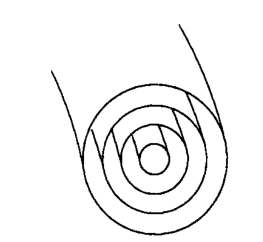
\includegraphics[width=0.95\textwidth]{figures/magnetic-flux-surfaces.png}
      \caption{Magnetic flux surfaces forming a set of nested toroids. This is because $\mathbf{B}\cdot\grad p=0$, this conclusion comes from $\mathbf{j\times B}=\grad p$.}
    \end{subfigure}%
    \begin{subfigure}{0.45\textwidth}
      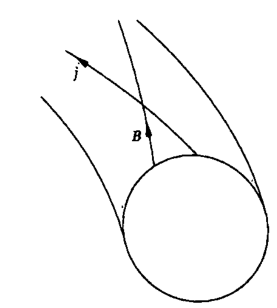
\includegraphics[width=0.95\textwidth]{figures/field-line-and-current-line.png}
      \caption{Magnetic field lines and current lines lie in magnetic surfaces. This is because $\mathbf{j}\cdot\grad p =0$.}
    \end{subfigure}
    \label{fig:magnetic-flux-surfaces}
  \end{figure}
\end{frame}

\begin{frame} {Grad-Shafranov Equation}
  The balance of tokamak requires $\mathbf{j\times B} = \grad p$. Using the flux function $\psi$, we are able to write it as
  \begin{equation}
    R\pdv{R}\,\frac{1}{R}\pdv{\psi}{R} + \pdv[2]{\psi}{z} = -\mu_0R^2p'(\psi) - \mu_0^2f(\psi)f'(\psi)
    \label{eq:grad-shafranov}
  \end{equation}

  \begin{figure}
    \centering
    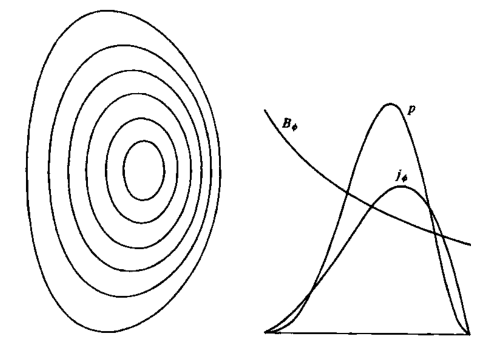
\includegraphics[width=0.5\textwidth]{figures/profiles.png}
    \caption{Euilibrium flux surfaces and plots of toroidal current density, plasma pressure, and toroidal magnetic field across the midplane.}
    \label{fig:profiles}
  \end{figure}
\end{frame}

\begin{frame} {Safety Factor, $q$}
  \begin{equation}
    q = \frac{\phi}{2\pi}
    \label{eq:safety-factor-definition}
  \end{equation}

  \begin{itemize}
    \item Plays important role in determining stability.
    \item $q$ characterize the number of winds of the $B$ field line goes around the plasma torus toroidally in one round of $\theta$.
  \end{itemize}

  Using $B_\phi$ and $B_p$ we can express safety factor as
  \begin{equation}
    q = \frac{1}{2\pi} \oint \frac{1}{R}\frac{B_\phi}{B_p}\dd{s}
    \label{eq:safety-factor}
  \end{equation}
  where $\dd{s}$ is the distance moved in $\theta$ direction while moving through $\dd{\phi}$. For large aspect-ratio tokamak of circular cross-section, we have approximation,
  \begin{equation}
    q = \frac{1}{2\pi} \oint \frac{1}{R}\frac{B_\phi}{B_p}\dd{s}
    \label{eq:safety-factor-large-aspect-ratio}
  \end{equation}
\end{frame}

\begin{frame} {Safety Factor, $q$ - Figures}
  \begin{figure}
    \centering
    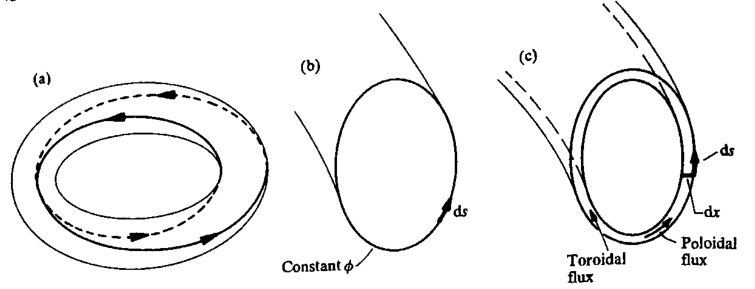
\includegraphics[width=0.95\textwidth]{figures/safety-factor.png}
    \caption{(a) Field line on $q=2$ surface. (b) Poloidal integration path for Eq.(\ref{eq:safety-factor}). (c) Flux annulus containing toroidal flux $\dd{\Phi}=\oint (B_\phi\dd{x})\dd{s}$ and poloidal flux $\dd{\Psi}=2\pi RB_p dx$}
    \label{fig:safety-factor}
  \end{figure}
\end{frame}

\begin{frame} {$q$ Profiles}
  The radial profile of $q$ is given by
  \begin{equation}
    q(r) = \frac{2B_\phi}{\mu_0\expval{j}_r R}
    \label{eq:radial-q-profile}
  \end{equation}
  where $\expval{j}_r = \int_0^rj(r')r'\dd{r'}/(r^2/2)$ is the average current density inside the radius $r$.

  \begin{itemize}
    \item An approximation: $q_{cyl} = 2\pi abB_\phi/\mu_0IR$.
    \item With $j=j_0(1-r^2/a^2)^\nu$,
          \[ q = \frac{2(\nu+1)}{\mu_0j_0}\frac{B_\phi}{R}\frac{r^2/a^2}{1-(1-r^2/a^2)^{\nu+1}} \]
          When near the X-point, the limiting form of $q$ as $d\to 0$ is
          \[ q\to \frac{B_\phi}{\pi R\abs{\grad B_p}}\ln\frac{\lambda}{d} \quad (d\to 0) \]
  \end{itemize}
\end{frame}

\begin{frame} {Beta}
  The efficiency of confinement of plasma is represented by the ratio
  \[ \beta = \frac{p}{B^2/2\mu_0} \]

  There are other slightly different definitions for different purposes,
  \begin{itemize}
    \item For a reactor, the important quantity is the thermonuclear power obtained for a given B field,
          \[ \beta^* = \frac{(\int p^2\dd\tau/\int\dd\tau)^{1/2}}{B_0^2/2\mu_0} \]
    \item A commonly used averaged beta
          \[ \expval{\beta}= \frac{\int p\dd\tau / \int\dd\tau}{B_0^2/2\mu_0} \]
    \item Poloidal $\beta$
          \[ \beta_p = \frac{\int p\dd{S} / \int\dd{S}}{B_a^2/2\mu_0} \]
          where the ingrals are surface integrals over the poloidal cross-section and $B_a = \mu_0I/l$.
  \end{itemize}
\end{frame}

\begin{frame} {Large Aspect-Ratio}
  For large aspect-ratio plasmas of circular cross-section with low $\beta$, the tokamak equilibria take a simple form.

  If the flux surface $\psi$ is displaced a distance $\Delta(\psi_0(r))$, $\psi$ may be written as
  \begin{equation}
    \psi = \psi_0 - \Delta(r)\cos\theta\dv{\psi_0}{r}
    \label{eq:psi-displaced}
  \end{equation}
  The Grad-Shafranov equation, Eq.(\ref{eq:grad-shafranov}), takes the form
  \begin{equation}
    \dv{r}\,\left(rB_{\theta0}^2\dv{\Delta}{r}\right) = \frac{r}{R_0}\left(2\mu_0r\dv{p_0}{r} - B_{\theta0}^2\right)
    \label{eq:grad-shafranov-large-aspect-ratio}
  \end{equation}
  Eq.(\ref{eq:psi-displaced}) and Eq.(\ref{eq:grad-shafranov-large-aspect-ratio}) together provide the solution $\psi(r,\theta)$.
\end{frame}

\begin{frame}{Large Aspect-Ratio - Figure}
  \begin{figure}
    \centering
    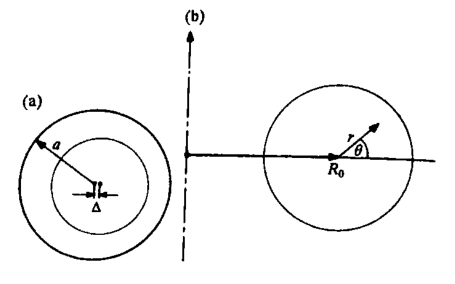
\includegraphics[width=0.7\textwidth]{figures/large-aspect-ratio.png}
    \caption{(a) Showing circular flux surface displaced by a distance $\Delta$ with respect to outer flux surface whose centre is at a distance $R_0$ from the major axis. (b) Coordinate system $(r,\theta)$ with centre at major radius $R_0$.}
    \label{fig:large-aspect-ratio}
  \end{figure}
\end{frame}

\begin{frame} {Shafranov Shift}
  The displacement $\Delta$ appears in Eq.(\ref{eq:psi-displaced}) is called the Shafranov shift.

  If the profiles of pressure and current are given by
  \[ p = \hat{p}\left(1-\frac{r^2}{a^2}\right),\quad
    j = \hat{j}\left(1-\frac{r^2}{a^2}\right)^\nu
  \]
  we can numerically solve the Shafranov shift $\Delta_s$, see Fig.\ref{fig:shafranov-shift}.
\end{frame}

\begin{frame} {Shafranov Shift}
  \begin{figure}
    \centering
    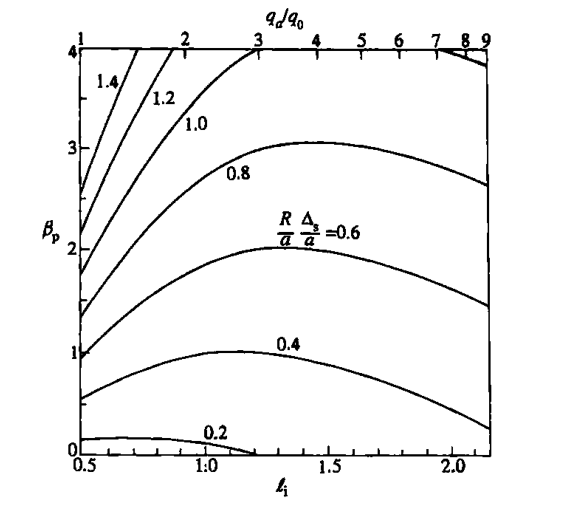
\includegraphics[width=0.5\textwidth]{figures/shafranov-shift.png}
    \caption{Graphs giving the Shafranov shift $\Delta_s$ in the form of contours of equal values of $(R/a)\Delta_s/a$ in the $(\beta_p,l_i)$ plane for a parabolic pressure profile and current profiles given by above, where $l_i=\overline{B_\theta^2}/B_{\theta a}^2$ is the internal inductance.}
    \label{fig:shafranov-shift}
  \end{figure}
\end{frame}

\begin{frame} {Vacuume Magnetic Field}
  The Eq.(\ref{eq:grad-shafranov-large-aspect-ratio}) enables us to determine the magnetic required to maintain the plasma equilibrium,

  \begin{equation}
    B_\theta(a) = B_{\theta0}(a)\left(1 + \frac{a}{R_0}\Lambda\cos\theta\right)
    \label{eq:poloidal-magnetic-field}
  \end{equation}
  where $\Lambda = \beta_p + \frac{l_i}{2} - 1$.

  The vaccume vertical magnetic field necessary to maintain the plasma in equilibrium is given by
  \[ B_v = -\frac{\mu_0I}{4\pi R_0}\left(\ln\frac{8R_0}{a}+ \Lambda - \frac{1}{2} \right) \]

  Its effect is to provide inward force to balance the outward hoop force on the plasma.
\end{frame}

\begin{frame} {Electric Field}
  This is just $\mathbf{j\times B}$
\end{frame}
